\chapter{Methodology}
\label{chap:method}

\section{Analysis of pyProCT}
\label{sec:sdd}

PyProCT uses \hyperref[sec:docs]{\textbf{pyScheduler} controller} to handle the execution of the algorithms . It features three modes: sequential, parallel, using python's multiprocessing module, and parallel using MPI. The refactor added a fourth mode to run the tool with pyCOMPSs. It is important to note that the modifications were limited to pyProCT, so COMPSs acts as a substitute of the current controller, not as a new scheduling method inside pyScheduler.


\subsection {Algorithms}

pyProCT uses the following five algorithms to find the best clustering. It also has an extra one which clusters the data randomly. This one is used for comparative purposes so it won't have more consideration that the utility it provides for other's behaviour analysis.

\begin{enumerate}

\item{K-medoids}
\item{Hierarchical}
\item{DBSCAN}
\item{GROMOS}
\item{Spectral}

\end{enumerate}

For more information about the actual implementation and parameter estimation of pyProCT check dropbox documentation on \ref{sec:docs} Documentation section.

\subsection{Execution Flow}
\label{sec:execution_flow}

The execution flow of pyProCT can be subdivided into four main sections linked to the JSON script structure:

\begin{description}
\item [Global,] \hfill \\ initialization of the software by reading parameters and options, parsing the JSON script, setting up the workspace and create the scheduler to be used.
\item [Data,] \hfill \\ construction of the distance matrix to be used. It offers three options: load, distance and rmsd.
\item [Clustering,] \hfill \\ calculation and evaluation of the clusterings.
\item [Postprocess,] \hfill \\ processing of the results to offer useful information about the clustering found.
\end{description}

On the next sections each part is going to be described, both it's execution flow and the json parameters associated with it.

\subsubsection{Global}

The global section is the responsible of initializing everything for the execution. This part is located on the main.py file and ends up calling the corresponding driver with the correct parameters. This is the main.py structure:

\begin{figure}[h]
\centering
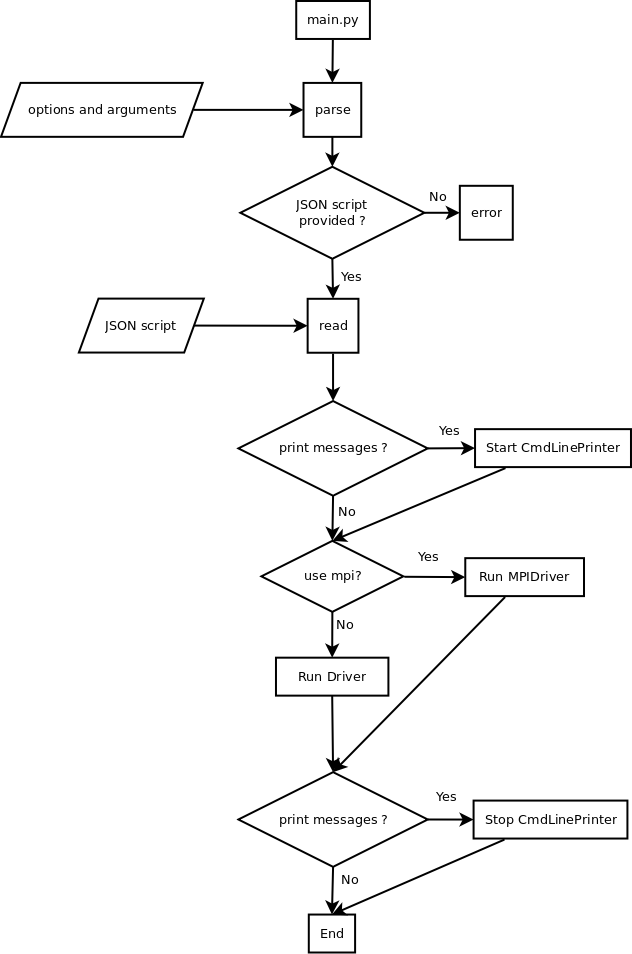
\includegraphics[height=0.5\paperheight]{img/global.png}
\caption{Global Section Execution Flow}
\vspace{1cm}
\end{figure}


This main file creates and initializes the Driver class which is the one orchestrating all the execution. Then the Driver class creates the workspace handler and saves the parameters before starting the Data, Clustering and Postprocess sections. The following figure shows encased in red the part corresponding to the global section inside the Driver. The next sections will expand the boxes Data, Clustering and Postprocess.

\begin{landscape}
\begin{figure}
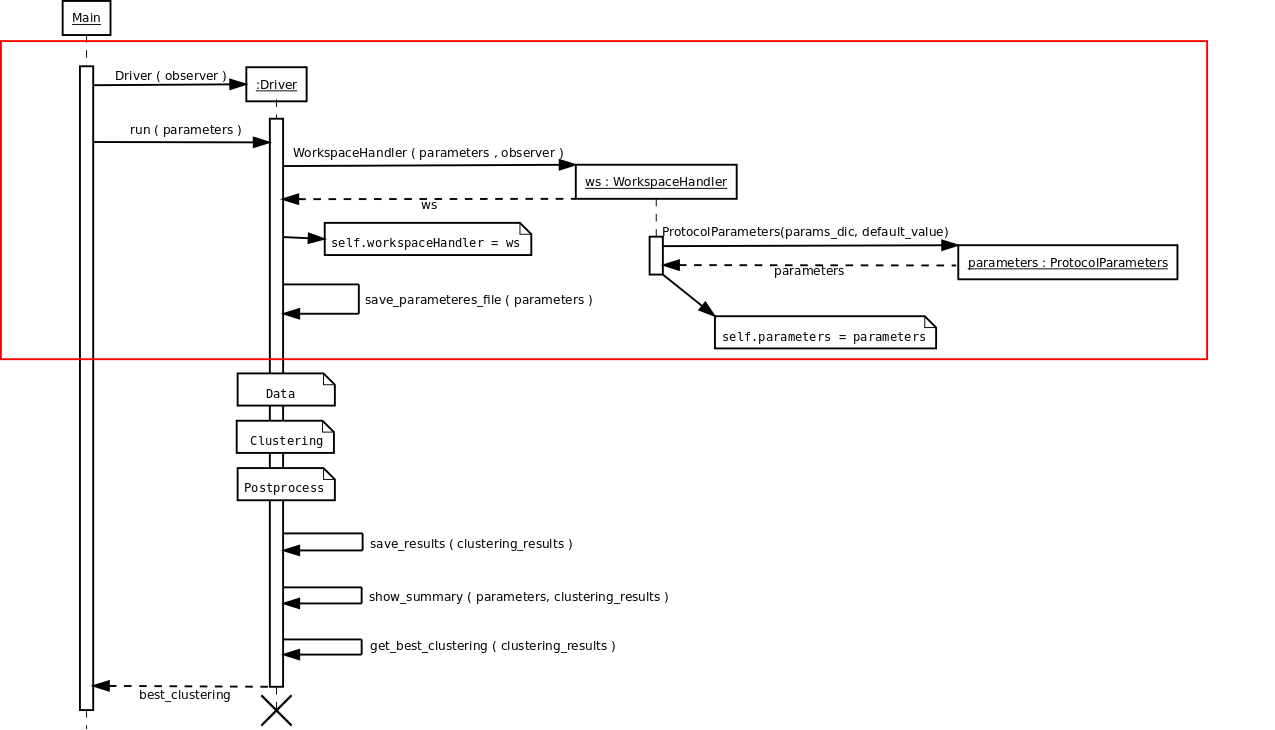
\includegraphics[width=25cm]{img/global_sequence_driver.jpg}
\caption{Global Section Execution Flow}
\end{figure}
\end{landscape}



The global section parameters that can be specified on the json file are divided into two groups: Control and Workspace. 

\begin{itemize}
\item \textbf{Control}
\begin{description}
\item [Scheduler type,] defines the kind of scheduler to use (serial, parallel, MPI or, after the refactor, pyCOMPSs)
\item [Number of processes,] if the parallel scheduler type is selected this option defines the number of processes to be used.
\end{description}
\item \textbf{Workspace}
\begin{description}
\item [Base,] is mandatory and defines the base workspace path.
\item [Tmp,] defines the folder to store temporal files.
\item [Matrix,] defines the folder to store the distance matrix (if applicable).
\item [Clusterings,] defines where cluster-related files are going to be stored, however the clusterings are stored as part of the results file.
\item [Results,] defines where the results file should be stored.
\item [Parameters:] \hfill
\begin{description}
\item [Overwrite,] if true, existing folders will be removed before execution.
\item [Clear after execution,] defines the folders to be removed after execution.
\end{description}
\end{description}
\end{itemize}


\subsubsection{Data}

This section defines how the distance matrix should be build. Essentially it runs the \textit{DataDriver}'s method \textit{run()} with the \textit{WorkspaceHandler} initialized on the global section and the retrieved parameters. This data driver initializes and returns to the main driver the \textit{DataHandler} and \textit{MatrixHandler} to be used later. The first one is directly instantiated with the corresponding parameters. The second one, on the other hand, first loads the matrix calculator defined on matrix's method of the json control file. With this calculator, the data handler and the parameters, it computes and returns the desired matrix handler. 

The following figure shows a simplified sequence diagram of this process:

\begin{landscape}
\begin{figure}
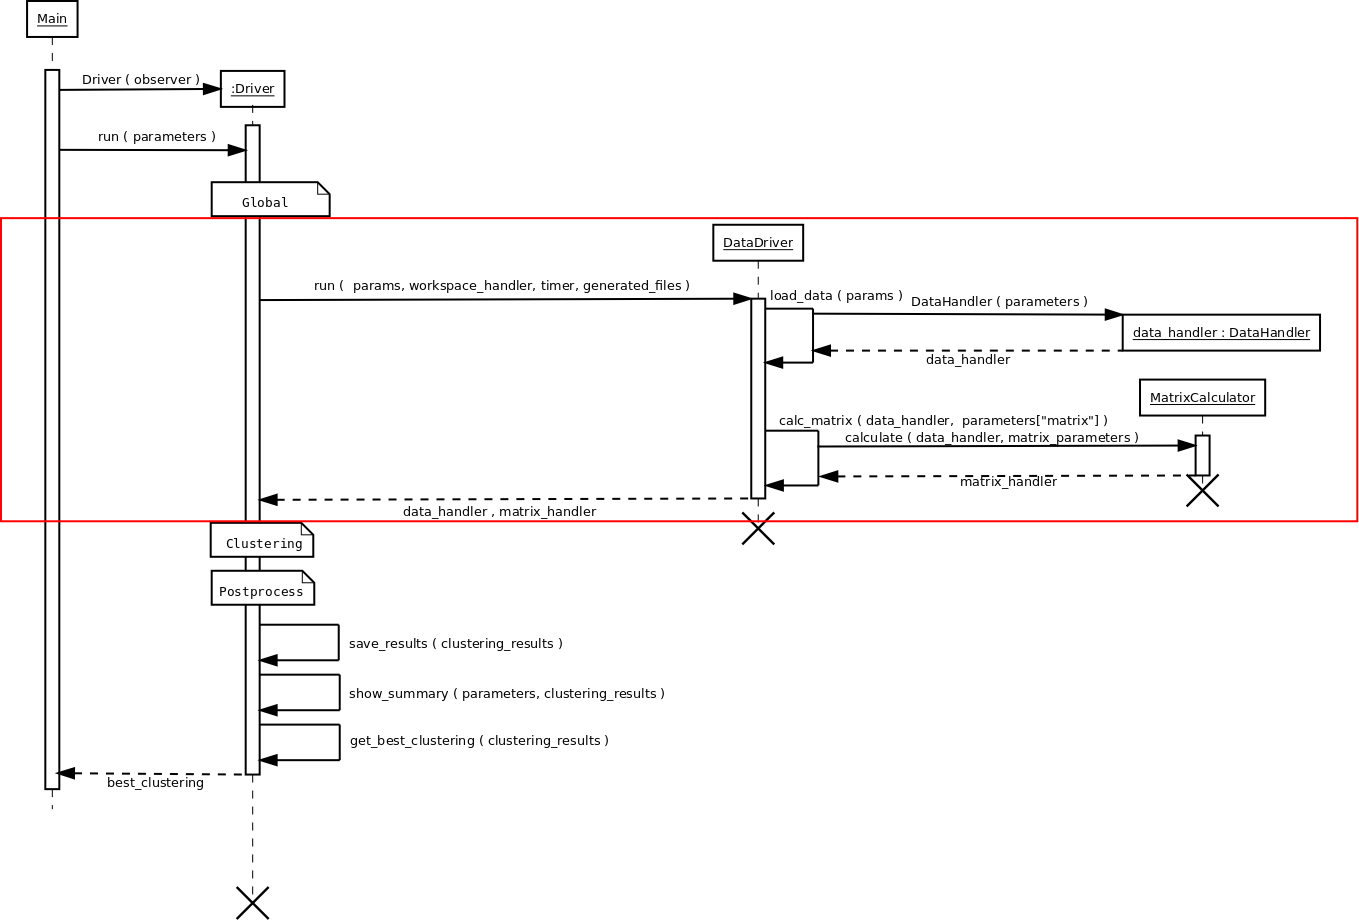
\includegraphics[width=24cm]{img/data_sequence_driver.png}
\caption{Data Section Execution Flow}
\end{figure}
\end{landscape}



The data section parameters specify the type and origin of the data, the method used to calculate the distance matrix and some more matrix-related parameters:


\begin{description}
\item [Type, ] sets the kind of data loader to use for the dataset.
\item [Files,] defines the location of the input files.
\item [Matrix] \hfil
\begin{description}
\item [Method,] selects the method used to calculate the distance matrix.
\item [Parameters,] allows to customize some parameters used to by the distance matrix calculator like:
\begin{description}
\item [Calculator Type,] must be one of the local pyRMSD installation available ones.
\item [Fit Selection,] for distance or rmsd methods.
\item [Body Selection,] for distance method.
\item [Calculate Selection,] for rmsd method.
\item [Path,] in case we are loading the matrix.
\end{description}
\item [Image,] setting this section will result in rendering a visual representation of the matrix.
\begin{description}
\item [Filename,] desired path of the rendered image.
\item [Dimension,] sets the leading dimension of the matrix image [default:1000px]
\end{description}
\item [Filename,] name of the file where the distance matrix will be saved (if applicable) inside the folder defined on workspace::matrix section. 
\end{description}
\end{description}


\subsubsection{Clustering}

This section is the one performing the actual clustering exploration and evaluation of the results. 

As \hyperref[fig:clustering_section]{Figure \ref{fig:clustering_section}} shows, the driver calls it's \textit{clustering\_section()} function which checks wether it needs to perform the exploration or load an existing clustering. 

If the method selected is "load" then the function \textit{from\_dic(...)} turns the data into a Clustering instance. 

If "generate" is the selected method then it calls \textit{perform\_clustering\_exploration(...)} which initializes and runs the \textit{ClusteringProtocol} class. This one, in turn, runs and initializes the classes  \textit{ClusteringExplorer}, \textit{ClusteringFilter}, \textit{AnalysisRunner} and the \textit{BestClusteringSelector}.

This clustering explorer deals with the actual exploration pipeline. It generates diverse parameter structures for each defined CA algorithm and adds them to the scheduler tasks queue, runs the scheduler and returns the resulting clustering\_info structures. 

The clustering filter tries to reduce the size of the clustering. To achieve this it eliminates the clusters whose parameters are outside the defined ranges on the evaluation section, removes the not selected clusters and checks that there are no repeated clusterings amongst the selected ones.

The analysis' runner is the one handling the evaluation of the selected clusterings. Similarly to \textit{ClusteringProtocol}, it creates an scheduler instance, queues the parametrization of each clustering analysis into it and runs it. Finally, it attaches the results to the clustering structure evaluated.

The BestClusteringSelector normalizes the calculated evaluations, scores each evaluation with the defined criteria and finally returns the id with higher score and the score itself.

Finally the ClusteringProtocol returns the clustering results containing:  \textit{best\_clustering\_id}, \textit{selected\_clusterings}, \textit{not\_selected\_clusterings} and \textit{all\_scores}. This results are then returned to the driver for the postprocessing section.

\begin{landscape}
\begin{figure}
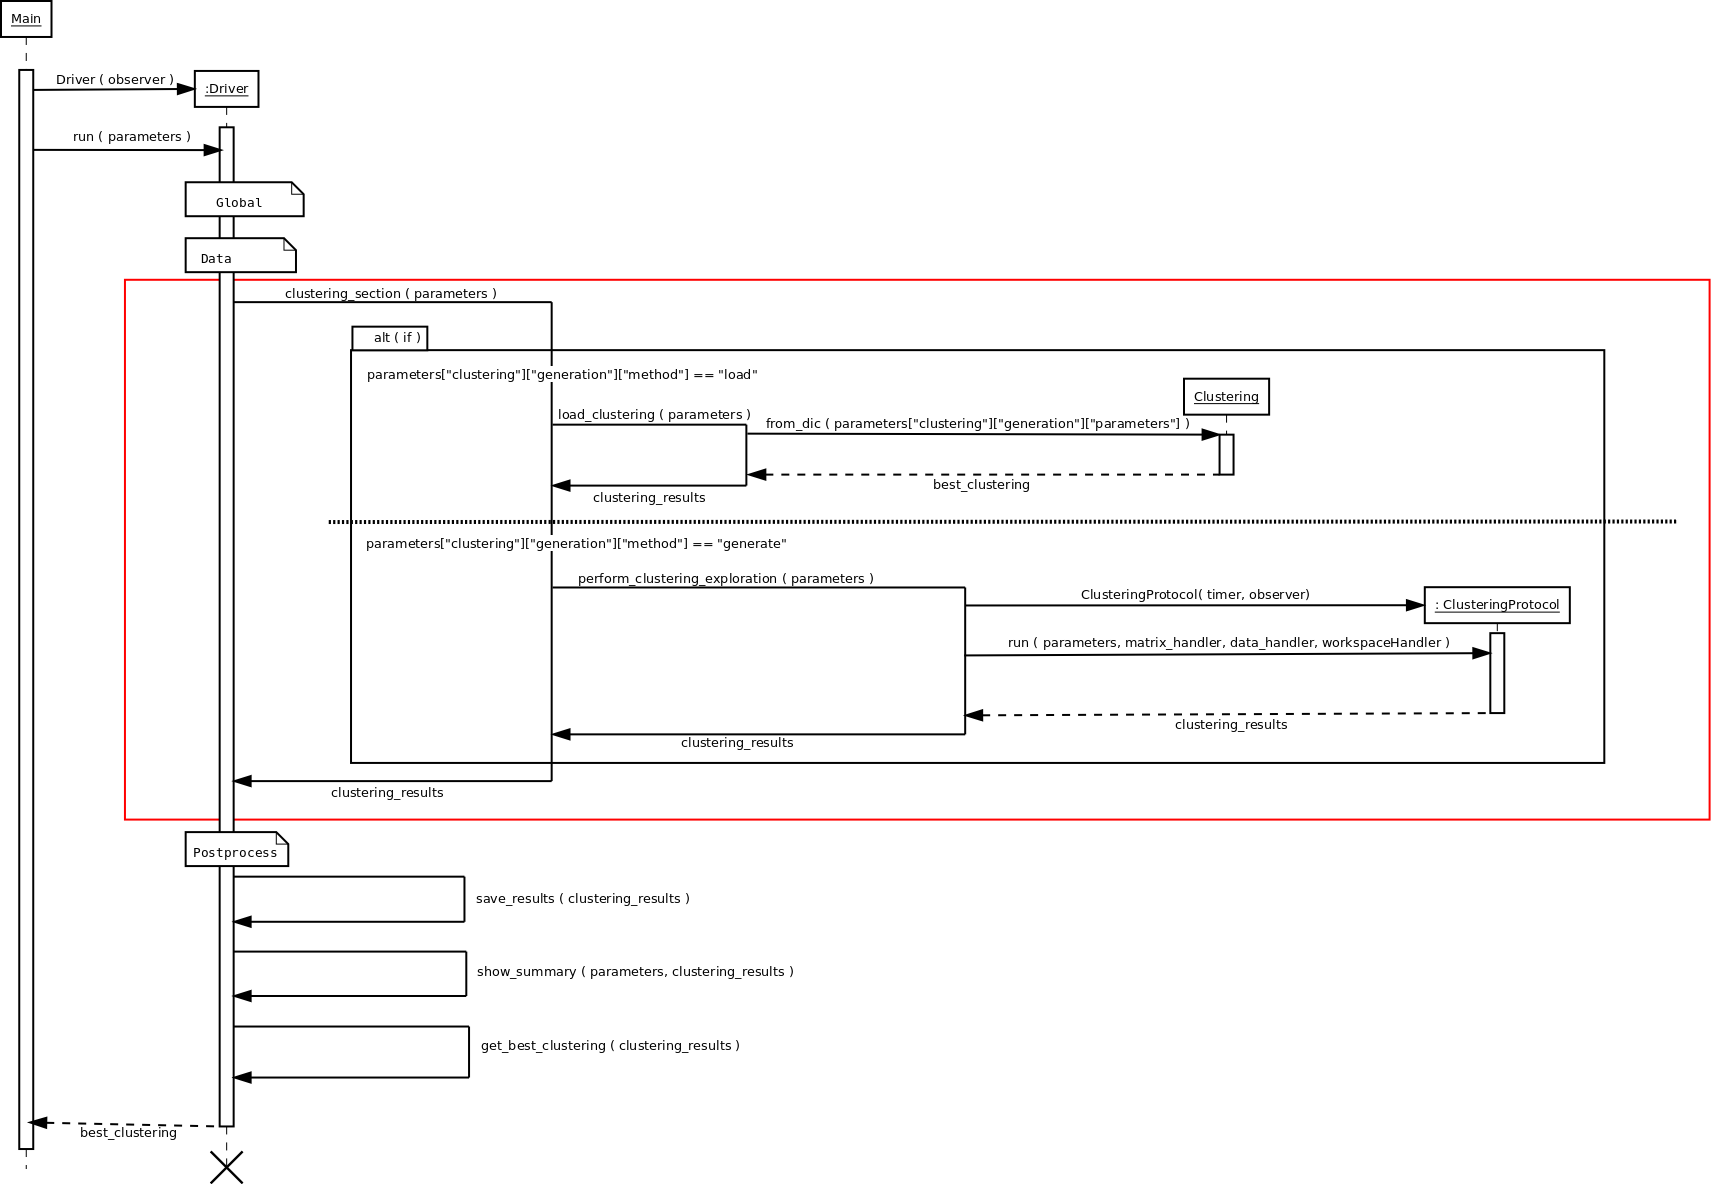
\includegraphics[width=24cm]{img/clustering_sequence_driver.png}
\caption{Clustering Section Execution Flow}
\label{fig:clustering_section}
\end{figure}
\end{landscape}



The clustering section parameters that can be specified on the json file define if the clustering should be generated or loaded, which algorithms and parameters to use and, finally, the evaluation section which is where the user should define his goal or hypothesis.

\begin{description}
\item [Generation] \hfil
\begin{description}
\item [Method,] selects wether we want to load or calculate the best clustering info. If it's loaded it will use the json dictionary defined on clustering::generation::clusters.
\item [Clusters,] clustering data if the method is "load". Each cluster object must define: id, prototype and elements.
\end{description}
\item [Algorithms,] \hfil \\for each desired algorithm to use of the six available (dbscan, gromos, hierarchical, kmedoids, random and spectral) defines it's parameters. All algorithms share the 'max', defining the maximim number of parametrizations for the algorithm, and the 'parameters' properties.
\begin{description}
\item [Kmedoids, ] \hfil 
\begin{description}
\item [Seeding type,] defines if the initial seeds should be randomly placed or at equidistant points.
\item [Tries,] if the initial seeds are to be randomly placed, this defines the number of repetitions done with different seeds (default: 10).
\end{description} 
\end{description}
\begin{description}
\item [Spectral, ] \hfil 
\begin{description}
\item [Sigma,] defines the sigma parameter for the spectral clustering. If not set, the default is to calculate local sigmas.
\end{description} 
\end{description}
\item [Evaluation] \hfil
\begin{description}
\item [Minimum clusters,] minimum number of clusters each clustering must contain to be evaluated.
\item [Maximum clusters,] maximum number of clusters a clustering must contain to be evaluated.
\item [Minimum cluster size,] any cluster smaller than this threshold will be considered noise (thus increasing the clustering noise).
\item [Minimum noise,] clusterings with higher noise than this threshold won't be evaluated.
\item [Query types,] list of details to be reported about the clustering found.
\item [Evaluation criteria,] list of criteria objects, each criteria containing one or more evaluation objects.
\begin{description}
\item [Evaluation object,] defines the sigma parameter for the spectral clustering. If not set, the default is to calculate local sigmas.
\begin{description}
\item [Name,] defining the quality function.
\item [Action,] defines wether the function should be maximized (">") or minimized ("<"). 
\item [Weight,] defines the relative weight of this quality function (not mandatory that they add up to 1).
\end{description}
\end{description} 
\end{description}
\end{description}



\subsubsection{Postprocess}

The postprocessing section's allows users to extract useful information about the clustering. This section is the only optional one amongst the four described. 

The Driver first gets the best clustering, which is the only remaining information needed to call the PostprocessingDriver class. The run method of this class loads all the available action classes and, for each one defined on the postprocessing section of the json file, runs it with the clustering information provided. The extracted information needs to be visualized with pyProCT GUI in some cases and saved into pdb files on the others (refer to \hyperref[subsec:postprocess:params]{Postprocessing Parameters} for more info)




\begin{landscape}
\begin{figure}
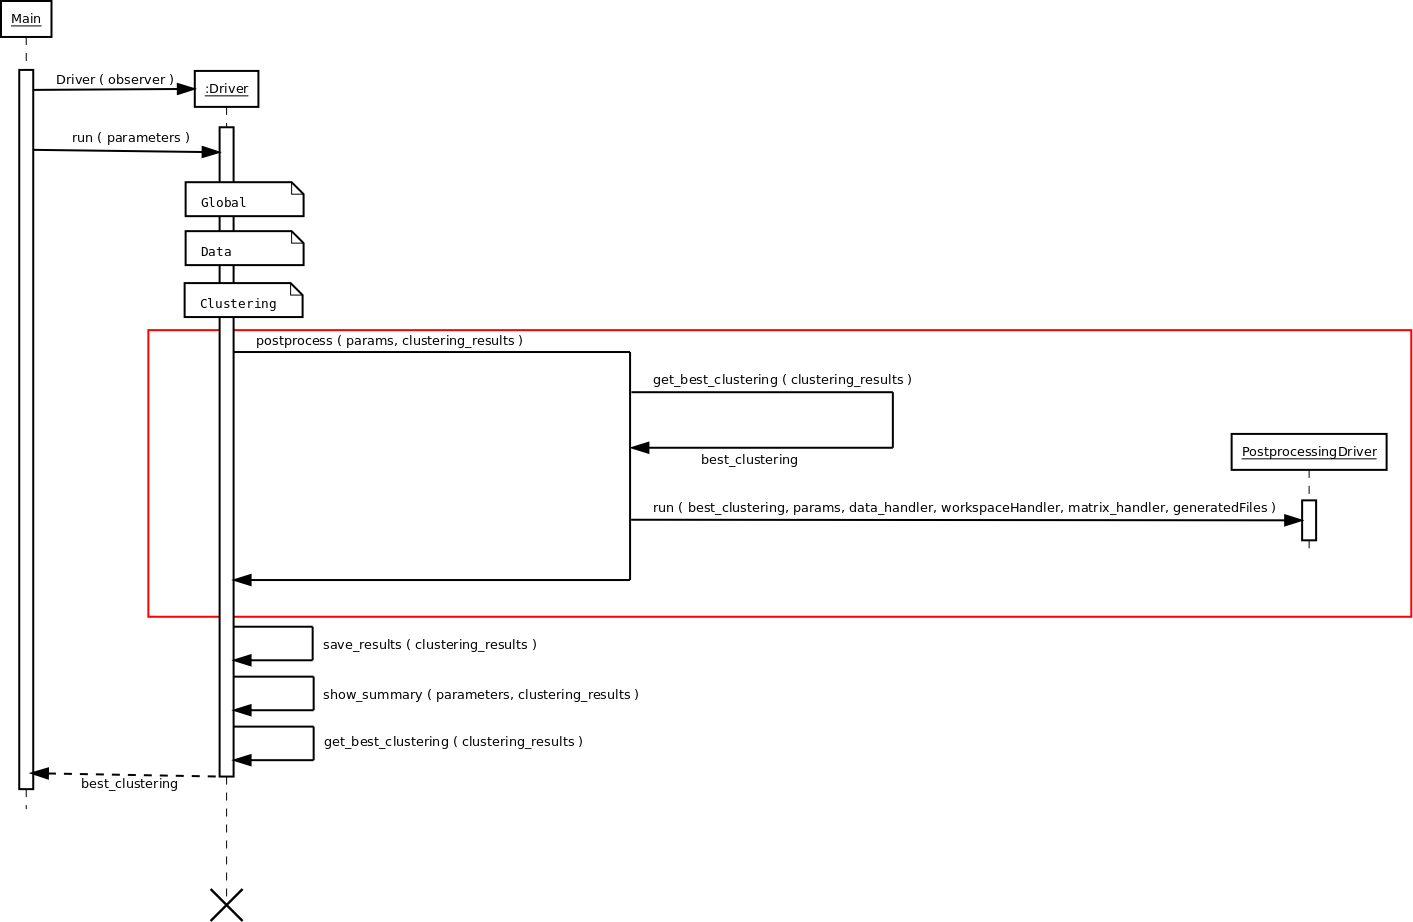
\includegraphics[width=24cm]{img/postprocess_sequence_driver.png}
\caption{Postprocess Section Execution Flow}
\end{figure}
\end{landscape}


\label{subsec:postprocess:params}
These are the possible postprocessing actions to be performed:


\begin{description}
\item [Rmsf,] pyProCT will generate the global and per-cluster
rmsf data to be visualized with the GUI.
\item [Centers and trace,] pyProCT will generate the data of all geometrical centers of the calculation selection of the system (to be visualized with the GUI)
\item [Representatives,] pyProCT will save the data of the medoid of each cluster on the best clustering in a pdb file.
\begin{description}
\item [Keep remarks,] if true, stored models will be saved with the their original remarks header (default: false).
\item [Keep frame number,] if set to true, the model number of any stored conformation will match the original pdb one (default: false).
\end{description}
\item [Pdb clusters,] pyProCT will save each cluster information in a pdb file.
\begin{description}
\item [Keep remarks,] if true, stored models will be saved with the their original remarks header (default: false).
\item [Keep frame number,] if set to true, the model number of any stored conformation will be the original pdb one. Default: false.
\end{description}
\item [Compression,] this option will produce a compressed version of the input trajectories with less redundancy thanks to the resulting clustering.
\begin{description}
\item [File,] name of the output file withouth extension (default:compressed.pdb)
\item [Final number of frames,] number of frames the compressed file must have.
\item [Type,] sampling method for cluster elements (default: kmedoids).
\begin{description}
\item [Random,] randomly samples elements for each cluster.
\item [Kmedoids,] uses k-medoids to get samples of the clusters.
\end{description}
\end{description}
\item [Cluster stats,] this will generate a human readable file with the distance among cluster centers and their diameters.  
\begin{description}
\item [File,] name of the generated file, without extension, to be stored inside results folder (default: per\_cluster\_stats.csv).
\end{description}
\end{description}



\section{Refactoring with pyCOMPSs}
\label{sec:refactor}

This section will walk you through all the refactor process. It will provide a full description of the issues found, wether they were solved or not, the design decisions made and the reasons behind them, and all the information relevant for debugging, testing and further developing both pyCOMPSs and pyProCT. 


\subsection{Set up}


The installation of pyProCT as described on the \hyperref[sec:docs]{pyProCT repo} is trivial on a local machine. On MareNostrum III pyProCT is already installed.  In order to use my version under development (instead of the package installed both on MN3 or a local machine) the user just needs to point the python path to it. This is useful to switch between different working versions (for example to use pyProCT-regression validation or to meet the different instrumentation requirements of each scheduler). Later some issues will also force me to use this same method to customize some of the dependencies of pyProCT such as the pyScheduler or pyRMSD. 

Choosing a good structure to set up the environment is a must for executions on MN3 because I faced and spent a lot of time on configuration problems. This kind of issues kept popping up during the whole project and are described on appendix XXXXXXXXXXX 



\subsection{pyCOMPSs}
\label{subsec:pycompss}

Prior to starting the refactor I analyzed which would be the best way to parallelize it. pyCOMPSs works by using python's decorators to define some functions as \textit{COMPSs' tasks}. These tasks are executed on previously defined resources such as a MN3 node or a cloud. For each task the framework checks whether that function's parameters depend on some previous task; if it has no dependencies then the task is assigned to a resource which runs it. 

pyProcT clustering and postprocessing sections, as previously stated, are embarrassingly parallel: all algorithm's executions depend only on the distance's matrix calculation; the postprocessing actions all depend on the best clustering (that is to say: the whole clustering section). Knowing this we decided to define as task each algorithm execution and each postprocessing action.

I wanted to maintain the possibility to use the other schedulers after the refactor so I kept the overall structure of pyProCT. However, I also wanted to exploit the possibility of reduce the code complexity while achieving the maximum performance improvement. I mention this because make the sequential version of pyProCT work with pyCOMPSs is enough to place the decorators on the right functions. It is true that this would also raise some issues to be addressed; my point is that the lines of code required are few if the goal is just to make it work. This is not the goal though. The refactor described from here onwards tries to minimize the code size, make it clearer. It also removes functionality duplication between the framework and the software. For example pyProCt has a loop which enqueues the tasks for the scheduler. COMPSs also has an internal queuing system rendering this loop unnecessary.

Bearing this in mind, differences are basically found on the Driver, Protocol and Explorer classes, which deal respectively with all the sections pipeline execution, the clustering pipeline, and the clustering exploration \textit{per se}. I simply created a new Driver for the COMPSs scheduling. The main checks whether pyCOMPSs is the scheduler or not and calls one driver or the other accordingly (same method being used for MPI). From the driver onwards the key classes are substituted by the COMPSs versions.

One of the advantages of pyCOMPSs is the small amount of work required to use it. On a normal sequential program we just need to use the \textit{@task()} decorator and the \textit{obj = compss\_wait\_on(obj)} API call to create synchronization points for future objects; from \hyperref[sec:docs]{COMPSs manual}: 

\begin{quote} 
If the programmer defines, as a task, a function or method that returns a value, that value is not generated until the task is executed. However, in order to keep the asynchrony of the task invocation, COMPSs manages future objects: a representant object is immediately returned to the main program when a task is invoked.
\end{quote}

Internally COMPSs has queue of tasks so the step to add the tasks to the scheduler is no longer required; instead I called directly the decorated methods (which internally COMPSs enqueues to it's pending's list). However this caused a problem related to the how the framework deals with the data.

To send the data needed by each task, that is, the method's parameters, COMPSs serializes them to files (except basic types). This means that python's pickle must be able to do the translation which is not the case for the distances matrix.

PyProCT uses pyRMSD \cite{Gil2013} (which stands for python Root Mean Squared Deviation) to represent the distances matrix. It is basically a python wrapper for a C matrix structure. The goal of this implementation is to highly reduce the access time to the matrix elements. 

\begin{quote}
Python is slow [...], why: it boils down to Python being a dynamically typed, interpreted language, where values are stored not in dense buffers but in scattered objects. \cite{vanderplas_why_2014}
\end{quote}

PyProCT overcomes this with the lean and specialized pyRMSD. The problem is that these structure is not a native python type nor it's built with a combination of them. Because of this the framework can not serialize this matrix to send it to each worker. The first idea to solve it was to dump the internal data of the matrix into a python list (which can be serialized arbitrarily) with the already implemented method \textit{get\_data}; this list then can be passed to the class constructor \textit{CondensedMatrix()} obtaining again the original one. This raised the question of where to perform the translation. 

The matrix's cast to a python list is linked to which is the function decorated as task. Before presenting working on it I inspected again how the algorithms are implemented and called. 

Each algorithm is implemented in a different class so we have \textit{kMedoidsAlgorithm.py}, \textit{spectralClusteringlAlgorithm.py} and so on. All of them however return the same kind of data: clusterings; in order to simplify all the execution pipeline and the code they all have the same structure: all the required arguments are passed to the class constructor and then they all have the \textit{perform\_clustering} method which returns the clusterings found for that parametrization. 

With this structure then it would be necessary to decorate the \textit{perform\_clustering} method of each algorithm but only when pyCOMPSs scheduling is used. In order to avoid having code duplication (one with the decorator and one without for each algorithm) I implemented a wrapper class, called CompssTask, for the algorithm's execution with a single pyCOMPSS-decorated method.

The class is constructed with all the required information for the task execution. During the initialization I also do the forementioned translation of the matrix to a python list. After the constructor the run method, which is the actual pyCOMPSs task executed on a worker, recreates the Condensed Matrix from the python list and executes the algorithm's clustering method. 

After the execution of the algorithm it was necessary to again deassign the computed matrix because it is part of the class and, even if it's not a result, once the task is finished pyCOMPSs again tries to serialize the object and fails.



\section{Validation tool: pyProCT-regression}
\label{sec:regression}

pyProCT-Regression is the software designed to validate the pyCOMPSs refactor code. It implements the so-called black-box validation method. The validator will take a list of tests to perform. First we need to generate the expected results with the original version or pyProCT, then we'll run the same tests with the new version and make sure that the output matches the expected results.


pyProCT results depend on the parameters defined on the control script because we can select which results to save, which format, whether we want to save the computed matrix (and it's image) and so on (see \hyperref[sec:execution_flow]{Section \ref{sec:execution_flow}} for more info). Because of that the validator needs to be flexible, allowing to define more or less files to check. On the other hand, we have two different test scenarios: one is to validate the results of the original version against the refactor, and the other to validate the new scheduler against known results of the other schedulers.

To achieve this behaviour, Regression takes a test list as input with all the information it needs to check for each test scenario. 
Each test has the following attributes.

\begin{description}
\item [Name,] a unique test name.
\item [Description,] an small description of the test.
\item [Script,] defines the input script for the pyProCT execution. 
\item [Expected results dir,] is the folder containing the expected output and the files specified on files\_to\_check
\item [Files to check:] a list of the additional files that regression will check, together with the default ones: test.out and test.err.
\end{description}

If we run the tester with the "GENERATE" option it will, for each test, run the installed pyProCT with the defined control script and save the normal standard output and error as well as the "files to check" on the "expected results dir".

On the other hand, running the tester with "TEST" will also run the control script with the installed pyProCT but after that it will check that the generated output matches the content of the "expected results dir".

The last three attributes allow us to use a single expected results directory with different scripts and schedulers, or use the new version of pyProCT with the same tests but on testing mode to validate the refactor. When validating that the original schedulers work as expected I also add other files to check such as the parameters.json and the clustering folders (containing information about the generated clustering).

\subsection{Basic tests and issues}

The basic tests validate each of the four sections of pyProCT (global, data, clusering, postprocess) incrementally. However once I started generating the MPI results I faced the first issue: MPI (and later also pyCOMPSs) scheduler need to be called with mpirun and runcompss. 

To solve it I could make all the schedulers work with the same call or adapt the tester to each scheduler (reading that information from the control script). I decided on the first because the scheduler is set on the control data (so the main file can act as a switch performing the runcompss of mpirun if needed) and pyProCT will be easier to use. Now the main file calls the bash script with the runcompss [params] and mpirun [params]. This way all the versions work same way and the tests on Regression just need to change the control script.

Once done this modifications it was easier to write the tests. Before starting the refactor I generated all the expected results. I tested this results with the same code that generated them to make sure the tester worked but some of them failed because of the second, and expected, issue: the random initializations of some algorithms. To solve this I did the same that on tic-tac-toe, albeit a bit more complex: "set the seeds" for the algorithm's initializations removing the stochastic and non-deterministic parts.

Afterwards, for each scheduler I ran the basic tests, first with the original pyProCT, then with the refactor. However the pyCOMPSs mode was not available before the refactor so I validated it's output against the expected results of the MPI (could be any of the others). pyCOMPSs embeds the application output on its own so, in this case, the tester checks if the expected output is contained within the pyCOMPSs one.

Finally for each major modification of pyProCT I ran this suite of tests to validate the work done.
